\vspace*{1.5pc}

It is expected that spatial homogeneity and isotropy break down on some scale. However, it is empirically verified that the Universe is \emph{statistically} homogeneous and isotropic. Take a look at the distribution of galaxies on the background figure on page~\pageref{chap:structure} for instance. At first glance, the cosmological principle holds: the distribution of large scale structures appears to be the same in whatever direction from the center you look in. In terms of spatial averages, the background distribution is in practical terms homogenous. But average out the distribution in smaller and smaller patches anywhere on the map and you may start to notice some dissimilarities from one patch to another of same dimensions. On really small scales, the distribution could hardly be more heterogenous: in some tiny patches, you may end up with a bunch of clumps or clusters of galaxies while in other barely if any. The characterisation of these inhomogeneities as one averages out over shorter and shorter volumes is grounded in a mathematical concept called the \textbf{power spectrum}. The wider the patch on which we average, the less of them we can place in our total available volume. This sampling variance --- or cosmic variance --- makes our statements about the largest of scales statistically less robust than on smaller scales since we cannot compare the entire observable Universe to anything else ! This won't limit our appreciation of the power spectrum as a powerful tool to probe large scales structures however, since we've already settled the global background evolution.

%%%%%%%%%%%%%%%%%%%%%%%%%%%%%%%%%%%%%%%%%%%%%%%%%%%%%
\subsection{Power Spectra: Definition}
%%%%%%%%%%%%%%%%%%%%%%%%%%%%%%%%%%%%%%%%%%%%%%%%%%%%%

\subsubsection{Inhomogeneities}

To study inhomogeneities in a generic density field $\varepsilon (\vec{x}, t)$, we can expand it to a mean value $\bar{\varepsilon} (t) = \langle \varepsilon(\vec{x},t) \rangle$ averaged over a hypersurface of simulatenity at time $t$ and a density contrast $\delta_\varepsilon$ in the field, large or small:
\begin{equation}
\label{eq:field}
\varepsilon(\vec{x}, t) = \bar{\varepsilon} (t) \left( ~1 ~+~ \delta_\varepsilon (\vec{x}, t) ~ \right)
\end{equation}
In the framework of cosmology, we will use conformal time $\tau = a^{-1} t$ instead of proper time and work in Fourier space\footnote{this is useful because each mode can be treated as evolving independantly of one another}, in which $\vec{\nabla}_{\vec{x}} \rightarrow - i \vec{k}$ and
\begin{equation}
\label{def:fourier}
\tilde{\varepsilon} (\vec{k}, \tau) = \mathcal{F}\left[ \varepsilon (\vec{x}, \tau) \right] = \int \frac{d^3 x}{(2 \pi)^3}~ \varepsilon(\vec{x}, \tau) e^{-i \vec{k} \cdot \vec{x}}
\end{equation}\\
It is clear from Eq.~\ref{eq:field} that the mean value of the field makes the average of the contrast null when averaged over a large enough volume. Making the time dependance implicit, we may characterize the variance in the field, by introducing
\begin{equation}
\label{def:ps_generic}
\left\{
\begin{array}{l}
\langle \delta_\varepsilon (\vec{k}) \rangle = 0\\
\\
\langle \delta_\varepsilon (\vec{k}) \delta_\varepsilon (\vec{k}^\prime) \rangle \doteq (2 \pi)^3~\delta^{\mathrm{(D)}} (\vec{k} - \vec{k}^\prime) \times P_\varepsilon (\vec{k})
\end{array}
\right.
\end{equation} where the Dirac distribution is defined as
\begin{equation}
\label{df:dirac_distrib}
\delta^{\mathrm{(D)}} (\vec{x}) = \left\{
\begin{array}{ll}
1 & \text{at}~ \vec{x} = \vec{0}\\
0 & \text{elsewhere}
\end{array}
\right.
\end{equation} $P_\varepsilon$ is known as the auto-correlation power spectrum of field $\varepsilon$, to distinguish it from the cross-correlation power spectrum of fields $\varepsilon$ and $\eta$, which is defined as
\begin{equation}
\langle \delta_\varepsilon (\vec{k}) \delta_\eta (\vec{k}^\prime) \rangle \doteq (2 \pi)^3~\delta^{\mathrm{(D)}} (\vec{k} - \vec{k}^\prime) \times P_{\varepsilon \eta} (\vec{k})
\end{equation}  It quantifies the contribution of each $\vec{k}$ vector mode to the field's variance and has the dimensions of a volume since $\vec{k}$ is the canonical conjugate of a spatial vector. When one considers a finite volume $\mathbb{V}$ with periodic conditions, the power spectrum can be interpreted as 
\begin{equation}
P_\varepsilon (\vec{k}) = \lim_{\mathbb{V} \rightarrow \infty} \frac{\langle \vert \delta_\varepsilon (\vec{k}) \vert^2 \rangle}{\mathbb{V}}
\end{equation} Assuming isotropy, the power spectrum does not depend on the direction $\hat{k} = \vec{k}/k$ but only on its magnitude $k = \vert \vec{k} \vert$: $P_\varepsilon (\vec{k}) = P_\varepsilon(k)$\\

\subsubsection{Anisotropies}

I will also consider fields which only depend on the relative orientation of momentum $\vec{p} = p \hat{p}$ with mode $\vec{k} = k \hat{k}$. Noting $\mu = \hat{p} \cdot \hat{k}$ the cosine of their relative angle, the relative fluctuation or contrast in field $\theta_X = \delta X / \bar{X}$ can be expanded into spherical harmonics
\begin{equation}
\label{eq:field_tensor}
\theta_X (\hat{k}, \mu) = \sum_{\ell = 1}^{\infty} \sum_{m = - \ell}^{+\ell} a^X_{\ell m} (\hat{k}, \mu) \mathcal{Y}_{\ell m} (\hat{p})
\end{equation} where
\begin{equation}
a^X_{\ell m} (\hat{k}, \mu) = (-i)^\ell 4\pi ~\iint d\Omega ~ \mathcal{Y}^{\ast}_{\ell m} (\hat{p}) \tilde{\theta}_X (\hat{k}, \mu)
\end{equation} and
\begin{equation}
\iint d\Omega ~\mathcal{Y}_{\ell m} (\hat{p}) \mathcal{Y}^{\ast}_{\ell^\prime m^\prime} (\hat{p}) = \delta_{\ell \ell^\prime} \delta_{mm^\prime}
\end{equation} The mean value being zero, the variance again defines a power spectrum. Here, the cross-correlation between $X$ and $Y$:
\begin{equation}
\label{eq:ps_ang_corr}
\left\{
\begin{array}{lcl}
\langle a^X_{\ell m} \rangle & = & 0\\
\\
\langle a^X_{\ell m} a^{Y,\ast}_{\ell^\prime m^\prime} \rangle  & = & \delta_{\ell \ell^\prime} \delta_{mm^\prime} \mathcal{C}^{XY}_\ell
\end{array}
\right.
\end{equation} where $\mathcal{C}_\ell$ has no dependance on $m$ because of  isotropy. $X$ and $Y$ can be scalar modes (\textit{e.g.} temperature) or tensor modes (\textit{e.g.} polarizations $+$ and $\times$, or $E$ and $B$). 



%%%%%%%%%%%%%%%%%%%%%%%%%%%%%%%%%%
\subsection{Matter Power Spectrum}
%%%%%%%%%%%%%%%%%%%%%%%%%%%%%%%%%%

\begin{figure}[!]
\begin{center}
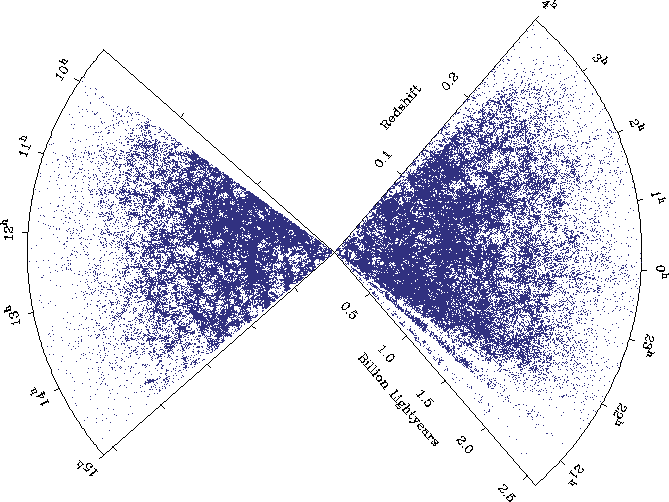
\includegraphics[height=5.5cm]{galaxies_2dFGRS_big.png}~%
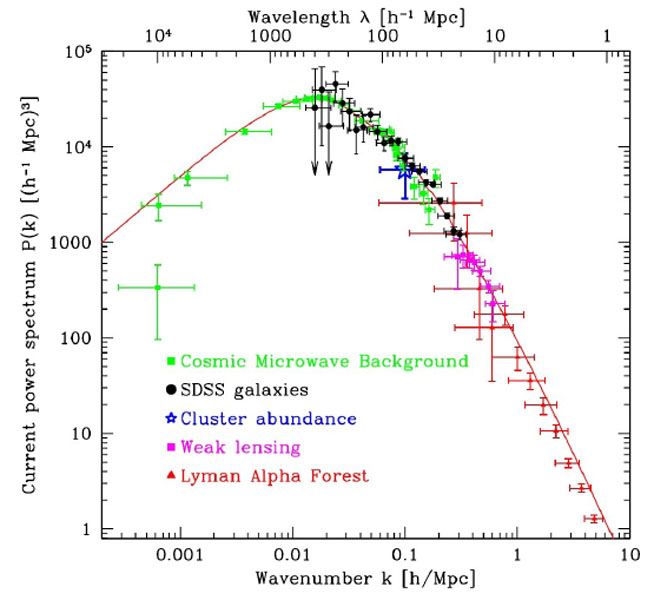
\includegraphics[height=5.5cm]{PS_z0.jpg}
\caption{\textbf{Left:} Distribution of galaxies within $2.5 \times 10^9$ light years of the Milky Way (center). Credit: 2dF Galaxy Redshift Survey. \textbf{Right:} Matter power spectrum measured at $z=0$ using 5 probes. The solid line is the best fitted $\Lambda$CDM model. Credit: \cite{PowerSpectrum_Tegmark}}
\label{fig:LSS}
\end{center}
\end{figure}

\subsubsection{Inhomogeneities in the Matter Distribution}

As I will detail in the next section, the density field of non-relativistic matter is only sensitive to monopolar perturbations, and so we may define the power spectrum of matter density contrast  at redshift $z$ as \\
\begin{empheq}[box=\mymath]{equation}
P_m (k, z) = \langle \vert \delta_m (k, z) \vert^2 \rangle
\end{empheq} \\ where
\begin{equation}
\delta_m (k, z )= \frac{\sum\limits_{i \in \lbrace cdm, b, \nu \rbrace} \bar{\rho}_i (z) \delta_i (k, z)}{\sum\limits_{i \in \lbrace cdm, b, \nu \rbrace} \bar{\rho}_i (z)}
\end{equation} when neutrinos are massive. The left-hand side of Eq.~\ref{def:ps_generic} for $\varepsilon = m$ is the auto-correlation function of non-relativistic matter. Since dark matter cannot be detected via electromagnetic waves, we can only infer its presence indirectly, using its impact on \emph{tracers}, \textit{i.e.} massive objects, commonly galaxies and quasars. It is clear from Eq.~\ref{def:ps_generic} that the power spectrum of these tracers and their correlation function $\xi(r)$ are a Fourier Transform pair
\begin{equation}
\xi (r) = \int \frac{d^3 k}{(2 \pi)^3} ~P(k)~ e^{i \vec{k} \cdot \vec{r}}
\end{equation} Because of isotropy, the correlation function is symmetric under rotation meaning it is only function of the relative position of objects $\xi(\vec{r}) = \xi(r)$, or equivalently $P(\vec{k}) = P(k)$. 
The power spectrum of these biased tracers can be linked to that of the underlying matter distribution by a real number $b \in \mathbb{R}$
\begin{equation}
P_{\mathrm{tracer}}(k) = b^2_{\mathrm{tracer}} P_m (k)
\end{equation} which is specific to the tracer used. When measuring the power spectrum of such a tracer, one must also take into account redshift distortion due to the peculiar velocity of the tracer which adds a Doppler shift (either blue-ward or red-ward) which skews the redshift along the line-of-sight. This anisotropy induced in the power spectrum is characterized by the Kaiser $\beta$ parameter \citep{Kaiser1987}:
\begin{equation}
P(k, \mu) = (1 + \beta ~\mu^2 k)^2 P(k)
\end{equation}\\

Finally, for objects on which we can only probe a density field along a line-of-sight such as for Lyman-alpha forests (see Sec.~\ref{sec:p1d}), it is useful to use the unidimensional power spectrum $P_{\mathrm{1d}}$ which is linked to the three-dimensional one by
\begin{empheq}[box=\mymath]{equation}
\label{eq:1dpwrspctrm}
\begin{array}{cl}
P_{\mathrm{1d}} (k_{\parallel}) &= \displaystyle \int \cfrac{d \vec{k}_{\bot}}{(2 \pi)^2}~ P_{\mathrm{3d}}(\vec{k}) \\
 &= \displaystyle \int \cfrac{dk}{2 \pi}~k P(k)
\end{array}
\end{empheq} where the mode vector $\vec{k} = (k_{\parallel}, \vec{k}_{\bot})$ is decomposed into a divergence-free (scalar) and a curl-free (vector) components. When not explicitely specified, $P(k) = P_{\mathrm{3d}}(k)$.\\


%It is helpful in computing the variance of $\delta$, since
%\begin{equation}
%\label{eq:variance_ps}
%\langle \delta^2 (\vec{r}) \rangle = \int_0^\infty \frac{dk}{k} \Delta^2 (k)
%\end{equation}
A very useful quantity to grasp the physical meaning of the power spectrum is the variance per logarithmic $k$, \textit{a.k.a.} the dimensionless power spectrum, defined as \\
\begin{empheq}[box=\mymath]{equation}
\label{eq:variance_ps}
\Delta^2 (k) \doteq \frac{k^3 P(k)}{2 \pi^2}
\end{empheq} \\ It is linked to the one-point variance of the density field 
\begin{align*}
\xi (r=0) &= \langle ~ \delta^2(0) ~ \rangle \\
&= \int \frac{\mathrm{d}^3\vec{k}}{(2 \pi)^3} ~ P(\vec{k}) \\
&= \int \frac{\mathrm{d}k}{2 \pi^2} ~ k^2 P(k) \\
&= \int \mathrm{d}\ln k ~ \frac{k^3 P(k)}{2 \pi^2} \\
&= \int \mathrm{d}\ln k ~ \Delta^2 (k)
\end{align*} To have a finite variance, which we assume to always have in cosmology, we require:
\begin{eqnarray}
\Delta^2 (k) \longrightarrow \left\{ \begin{array}{ccl}
0 &\text{as}& k \rightarrow 0\\
0 &\text{as}& k \rightarrow \infty
\end{array}
\right.
\end{eqnarray} In other words, if the power spectrum is polynomial $P(k) \sim k^n$, then, 
\begin{eqnarray}
n ~\left\{ \begin{array}{ccl}
> -3 &\text{as}& k \rightarrow 0\\
< -3 &\text{as}& k \rightarrow \infty
\end{array}
\right.
\end{eqnarray} Note that the power spectrum can diverge as $k \rightarrow 0$.\\



\subsubsection{Link with Real-Space Fluctuations}

Let $m(\mathbb{V}) = \displaystyle \int_\mathbb{V} \mathrm{d}^3 \vec{r} ~\rho(\vec{r})$ be the mass in a finite volume $\mathbb{V}$. The normalized mass fluctuation in volume $\mathbb{V}$ is defined as
\begin{equation}
\sigma^2 (\mathbb{V}) \doteq \frac{( m(\mathbb{V}) - \langle m(\mathbb{V}) \rangle)^2}{\langle m(\mathbb{V}) \rangle^2}
\end{equation} By substituting the density contrast and the auto-correlation of its field, it is straightforward to show that
\begin{equation}
\sigma^2_\mathbb{V} = \int \mathrm{d}^3 \vec{k} ~P(\vec{k})~ \vert W_\mathbb{V} (\vec{k}) \vert^2
\end{equation} where
\begin{equation}
W_\mathbb{V} (\vec{k}) = \frac{1}{\mathbb{V}} \int_\mathbb{V} \mathrm{d}^3 \vec{r} ~e^{i \vec{k} \cdot \vec{r}}
\end{equation} is the Fourier Transform of the following window function
\begin{eqnarray}
W_\mathbb{V} (\vec{r}) = \left\{ \begin{array}{cl}
1/\mathbb{V} &\text{where}~ \vec{r} \in \mathbb{V}\\
0 &\text{everywhere else}
\end{array}
\right.
\end{eqnarray} \\ In the case where $\mathbb{V}$ is a sphere of radius $R$, 
\begin{equation}
W_\mathbb{V} (\vec{r}) = \frac{3}{4 \pi R^3} ~\mathcal{H}(R-r)
\end{equation} where $\mathcal{H}$ is the Heavyside function. Computing its Fourier Transform
$$ \tilde{W}_R (\vec{k}) = \frac{3}{(kR)^3} ~ \left( \sin kR ~- kR \cos kR \right) $$ and assuming a power spectrum of the form $P(k) \sim A k^n$, the normalized mass function in the sphere of radius $R$ takes the form $$ \sigma^2(R) = 9AR^{-(n+3)} \int_{0}^{kR} d^3 y ~ y^{n-6} \left( \sin y - y \cos y \right)^2 $$ For $n>1$ on one hand, $\sigma^2 (R) \propto R^{-4}$. For $n<1$ on the other hand, the above integral converges as $kR \rightarrow \infty$ and
\begin{align*}
\sigma^2(R) &\propto AR^{-(n+3)} \\
&\propto \Delta^2 (k = R^{-1}) \\
&\propto \left[ k^3 P(k) \right]_{k=R^{-1}}
\end{align*} \\
For what follow, we will denote the mass variance within a co-moving radius of $R=8 ~h^{-1}$Mpc as
\begin{empheq}[box=\mymath]{equation}
\label{def:sig8}
\sigma_8 \doteq \sqrt{\sigma^2(R=8~h^{-1}\mathrm{Mpc})}
\end{empheq}


\begin{figure}
\begin{center}
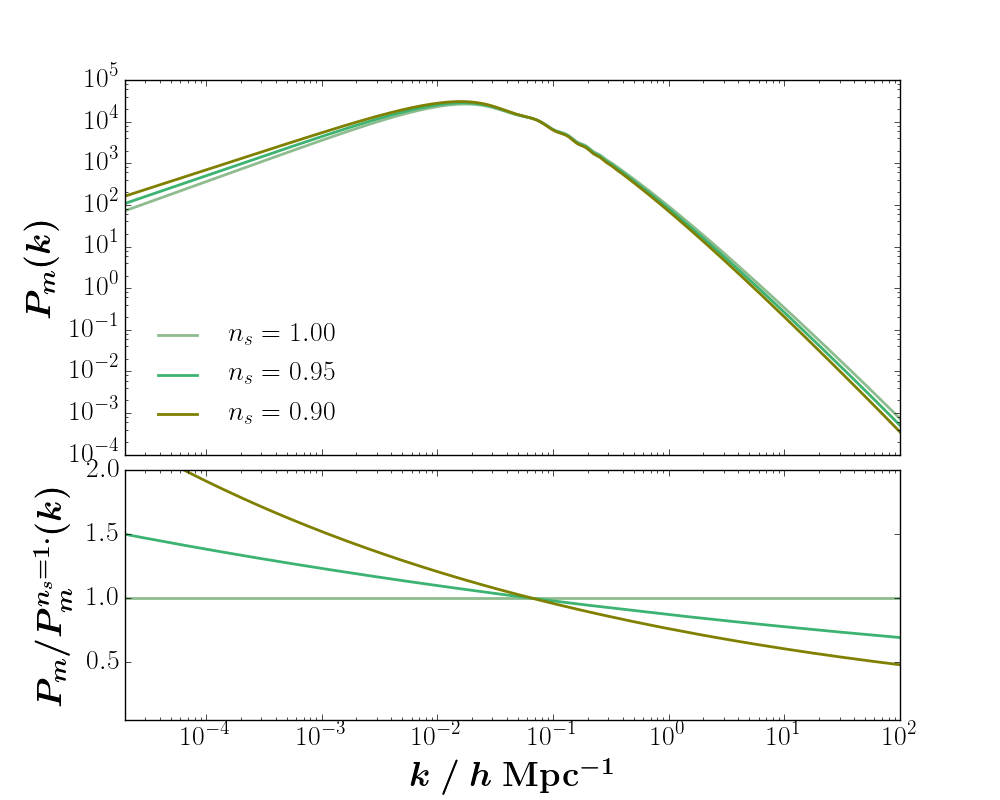
\includegraphics[width=0.65\linewidth]{CosmoParam/Pk_ns.png}
%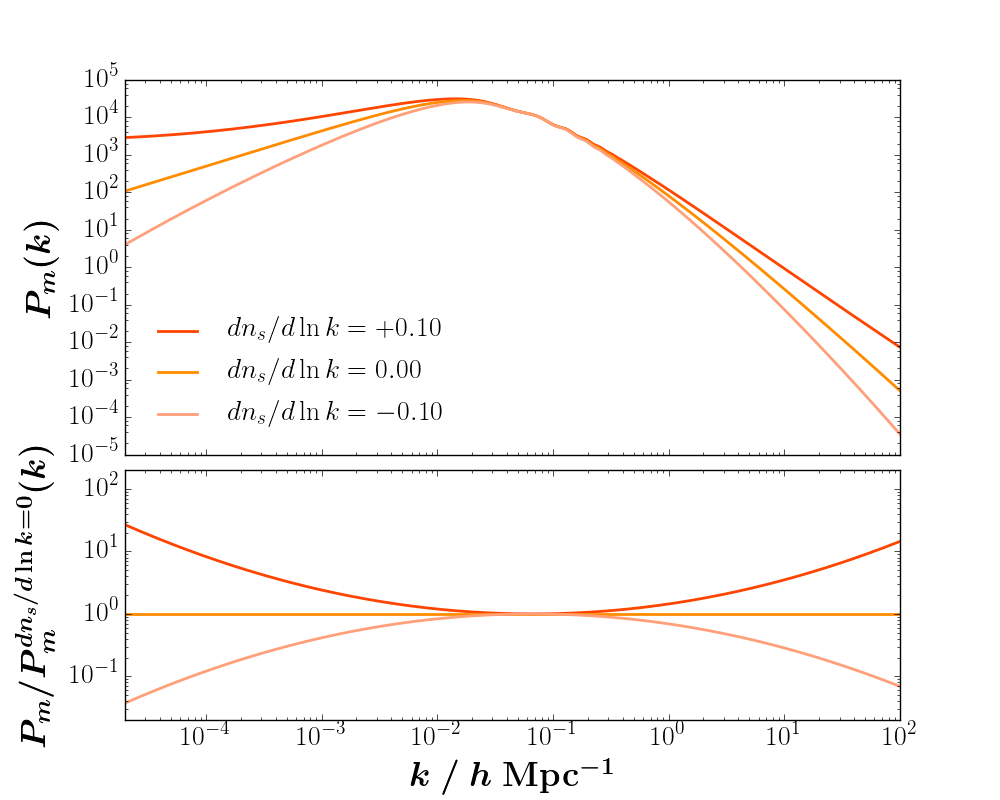
\includegraphics[width=0.4\linewidth]{CosmoParam/Pk_nrun.png}
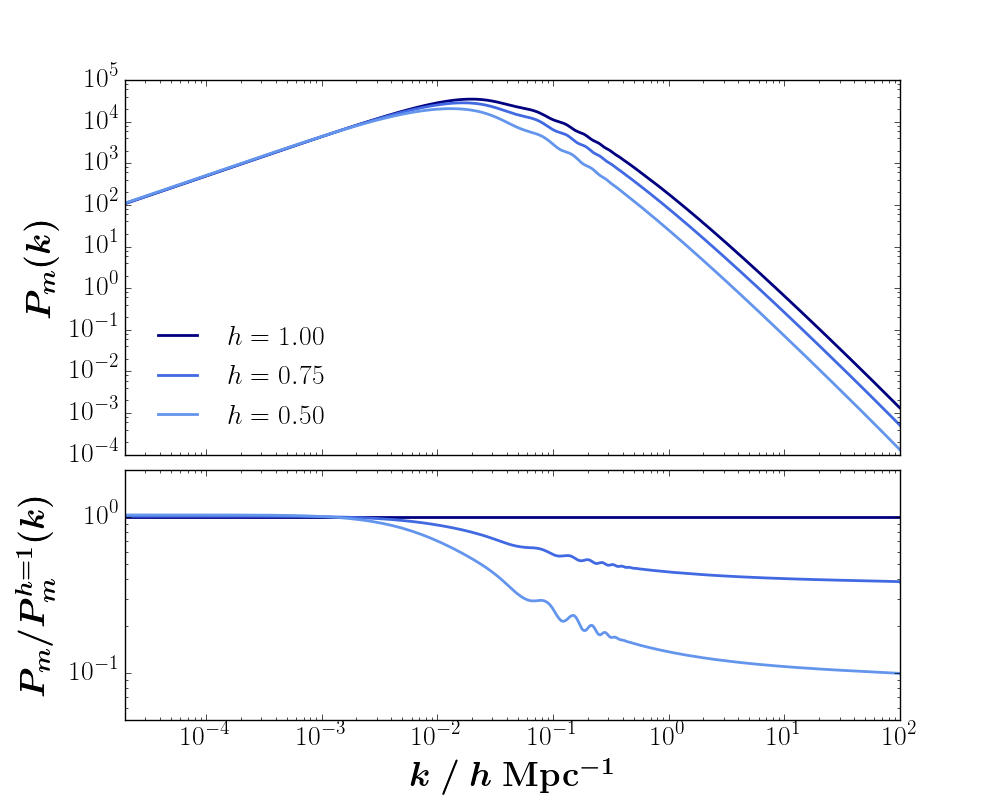
\includegraphics[width=0.65\linewidth]{CosmoParam/Pk_h.png}
%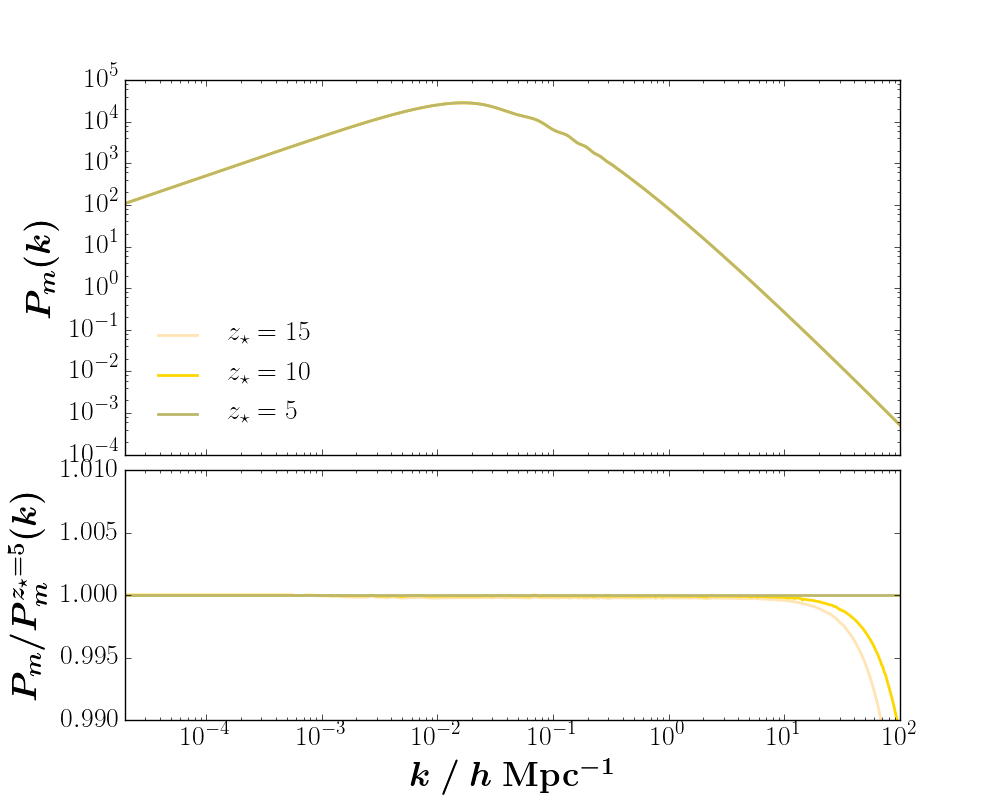
\includegraphics[width=0.4\linewidth]{CosmoParam/Pk_zreio.png}
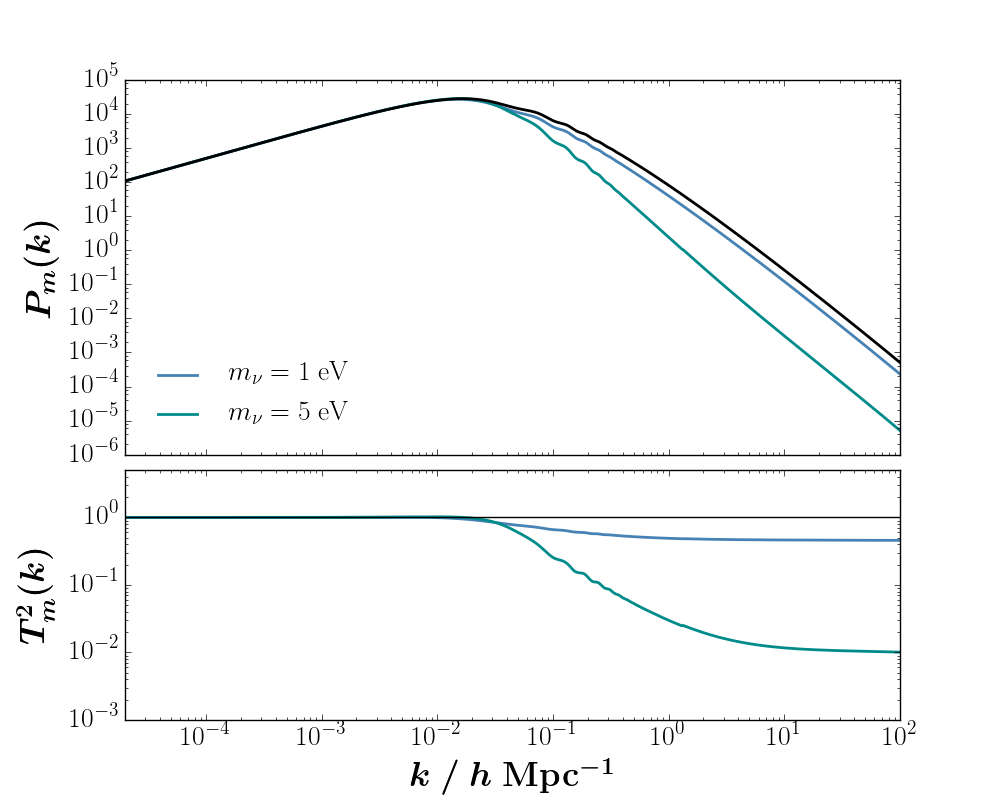
\includegraphics[width=0.65\linewidth]{CosmoParam/Pk_mnu.png}
%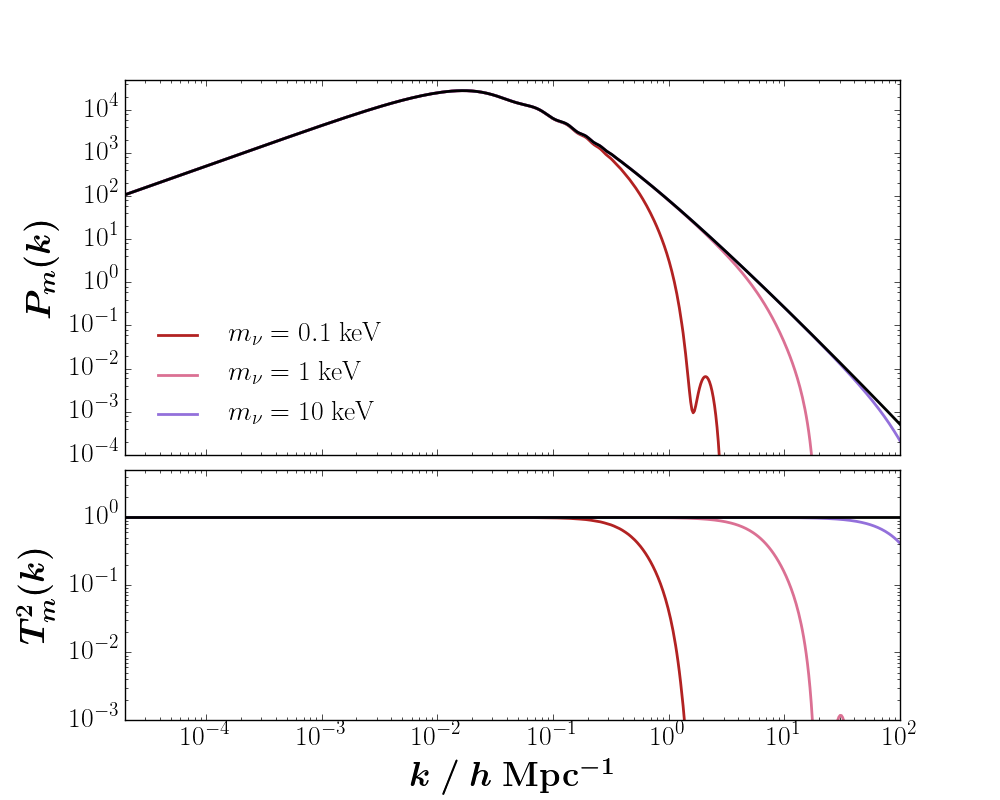
\includegraphics[width=0.4\linewidth]{CosmoParam/Pk_pdm.png}
\caption{Matter power spectrum at $z=0$ and their residual with respect to the standard values of the $\Lambda$CDM model, for varying values of the spectral index (\textbf{top}, see definition in Eq.~\ref{def:Harrison} and Sec.~\ref{sec:primordialps}), expansion rate (\textbf{middle}) and neutrino mass (\textbf{bottom}, see Sec~\ref{sec:mdmps}).}
\label{fig:Pk_cosmo}
\end{center}
\end{figure}


%%%%%%%%%%%%%%%%%%%%%%%%%%%%%%%%%%%%%%%%%%%%%%%%%%%
\subsection{Angular Power Spectrum of Anisotropies}
%%%%%%%%%%%%%%%%%%%%%%%%%%%%%%%%%%%%%%%%%%%%%%%%%%%

\begin{figure}[!]
\begin{center}
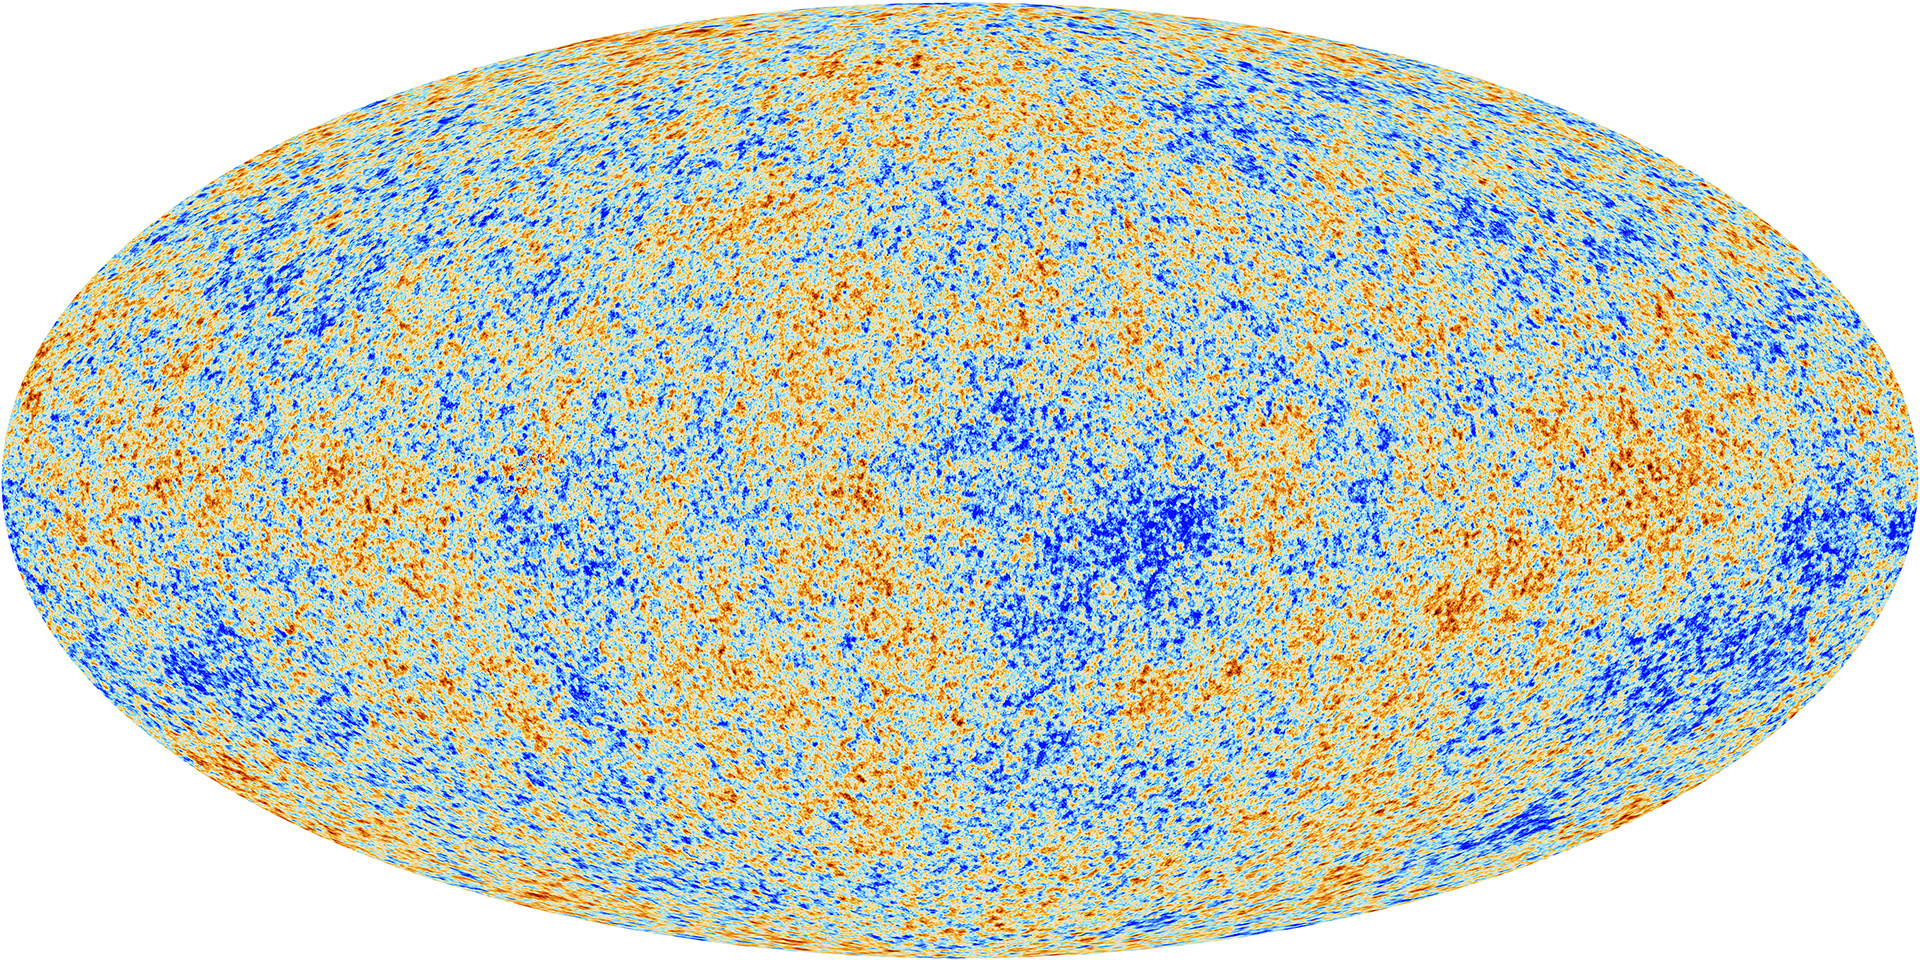
\includegraphics[height=5cm]{Planck_CMB.jpg}~%
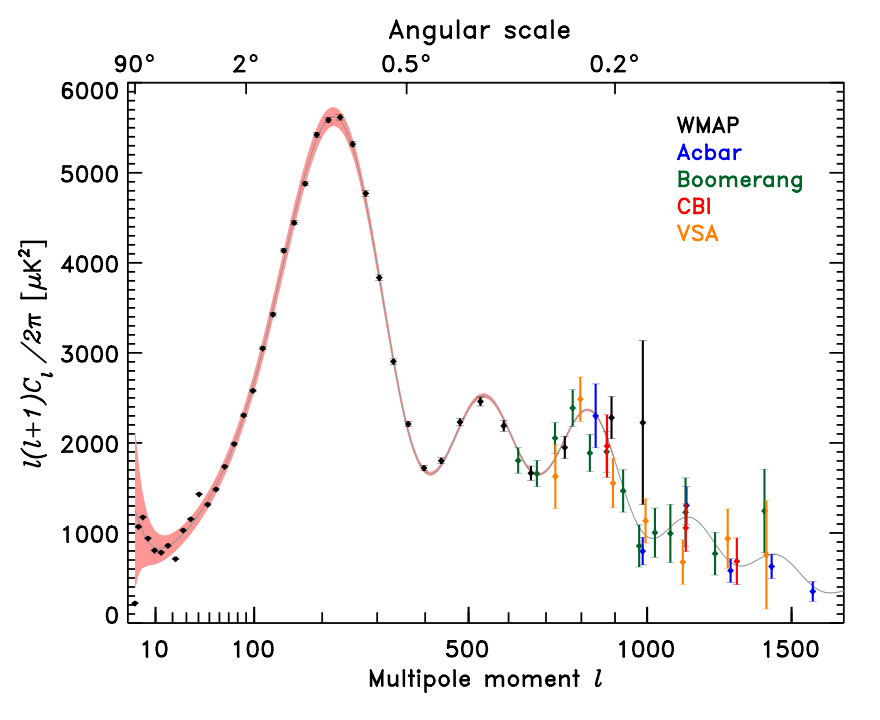
\includegraphics[height=5.5cm]{CMB_PS.png}
\caption{\textbf{Left:} Mollweide projection of the CMB temperature anisotropies taken by the Planck spacecraft, year 2. Credit: Planck. \textbf{Right:} Angular power spectrum of temperature anisotropies measured by 5 experiments.}
\label{fig:CMB}
\end{center}
\end{figure}


\subsubsection{Anisotropies in the Temperature Distribution}


Replacing $X$ and $Y$ in expressions~\ref{eq:field_tensor} by the fluctuation in temperature $T_\gamma$ of CMB photons, \\
\begin{equation}
T(\hat{p}, \tau) ~=~ \bar{T}(\tau) ~\left( 1 + \theta(\hat{p}, \tau) \right)
\end{equation} \\ Eq.~\ref{eq:ps_ang_corr} gives the angular auto-correlation power spectrum in temperature fluctuations. The harmonic modes $\mathcal{Y}_{\ell m}$ quantify the temperature fluctuations on solid angle $\Delta \Omega \sim \pi / \ell$. The $00$ harmonic is therefore the CMB temperature averaged over the entire sky: \\
\begin{equation}
a^{\theta \theta}_{00} = 2.72548 \pm 0.00057 ~\mathrm{K} 
\end{equation} \\ as computed in \cite{Fixsen2009}. The first harmonic (dipole) $\ell = 1$ is dominated by the solar system's relative velocity with respect to the CMB, measured in \cite{Lineweaver1996a} to be \\
\begin{equation}
a_{10} =  3.358 \pm 0.023 ~\mathrm{mK}
\end{equation} \\ To study the relative importance of the various harmonics, one can look at the variance of the temperature anisotropies, \\
\begin{equation}
\langle \vert \theta \vert^2 \rangle = \frac{1}{4 \pi} \sum_{\ell = 2}^{\infty} (2 \ell +1) \mathcal{C}_{\ell}
\end{equation} \\ using the orthonormalisation relation of the spherical harmonic base. Just as we defined the variance per log $k$ of the matter power spectrum, which related to the variance in density contrast, we similarly often consider the quantity \\
\begin{empheq}[box=\mymath]{equation}
\mathcal{D}_\ell = \Delta^2_\theta (\ell) = \frac{\ell (\ell + 1)}{2 \pi} \mathcal{C}_\ell
\end{empheq} which quantifies the variance in temperature contrast at a give angular scale $\ell \sim \pi / \Omega$. 


\subsubsection{Link With Matter Power Spectrum}

It can be shown that the temperature anisotropy field can be linked to the overdensity field via
\begin{equation}
\langle \theta(\vec{k}, \hat{p}) \theta^{\ast}(\vec{k}^\prime, \hat{p}^\prime) \rangle = \langle \delta(\vec{k}) \delta^{\ast} (\vec{k}^\prime) \rangle ~\times~ \frac{\theta(k, \hat{k}\cdot \hat{p})}{\delta(k)}~\frac{\theta^{\ast}(k, \hat{k}\cdot \hat{p}^\prime)}{\delta^{\ast}(k)}
\end{equation} which establishes a link between the matter power spectrum and the $\mathcal{C}_\ell$:

\begin{equation}
\mathcal{C}_{\ell} = \frac{2}{\pi} \int_{0}^{\pi} dk~k^2 P(k) ~\left\vert \frac{\theta_{\ell} (k)}{\delta(k)} \right\vert
\end{equation}

\begin{figure}
\begin{center}
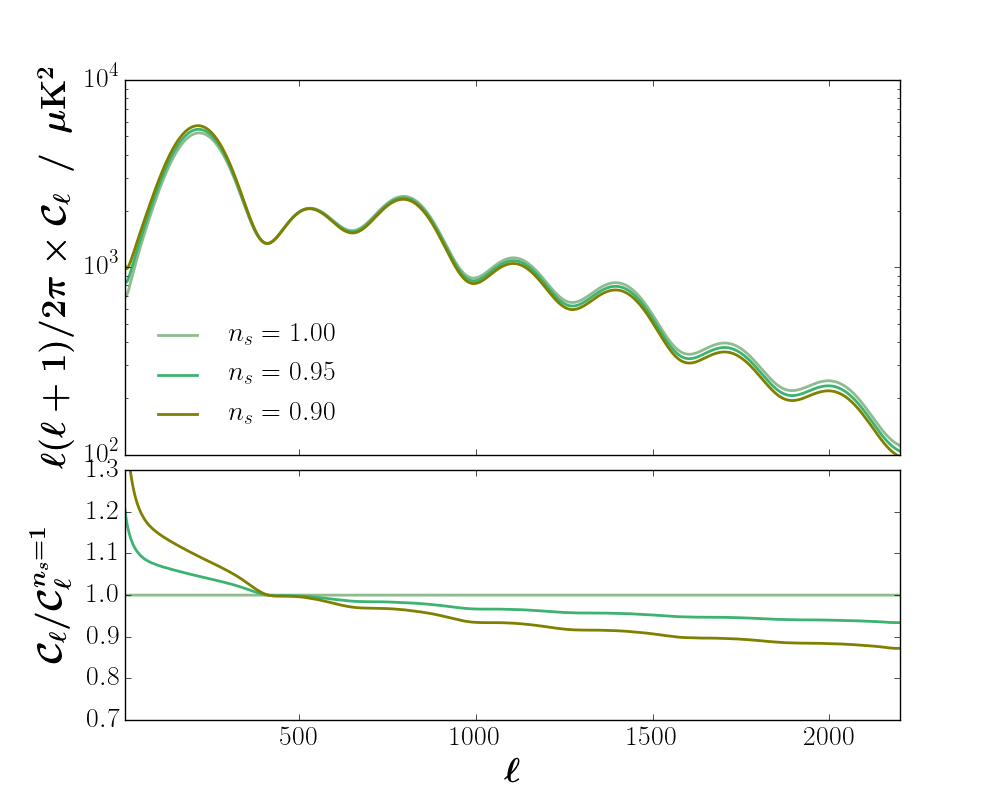
\includegraphics[width=0.65\linewidth]{CosmoParam/Cell_ns.png}
%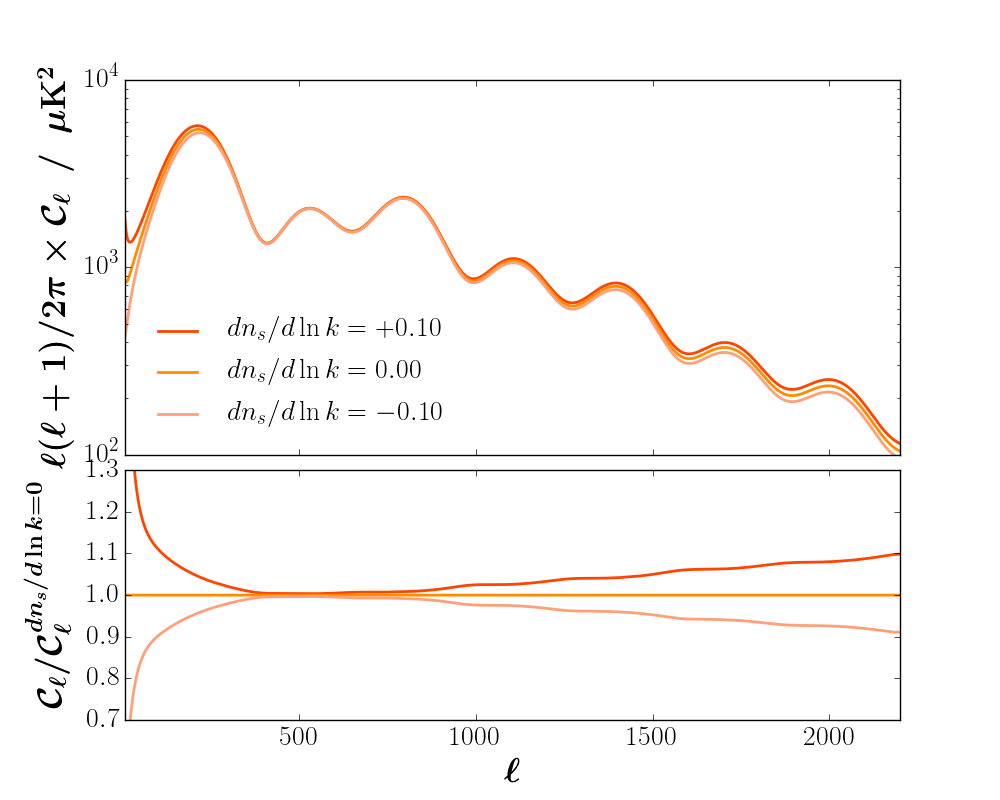
\includegraphics[width=0.45\linewidth]{CosmoParam/Cell_nrun.png}
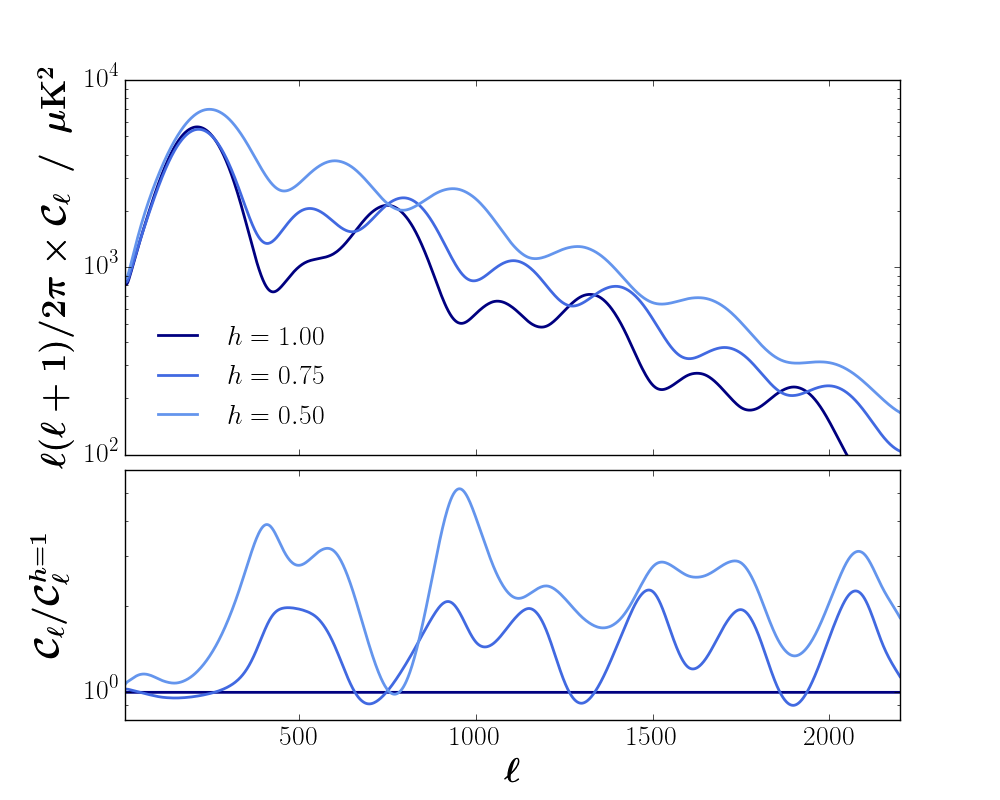
\includegraphics[width=0.65\linewidth]{CosmoParam/Cell_h.png}
%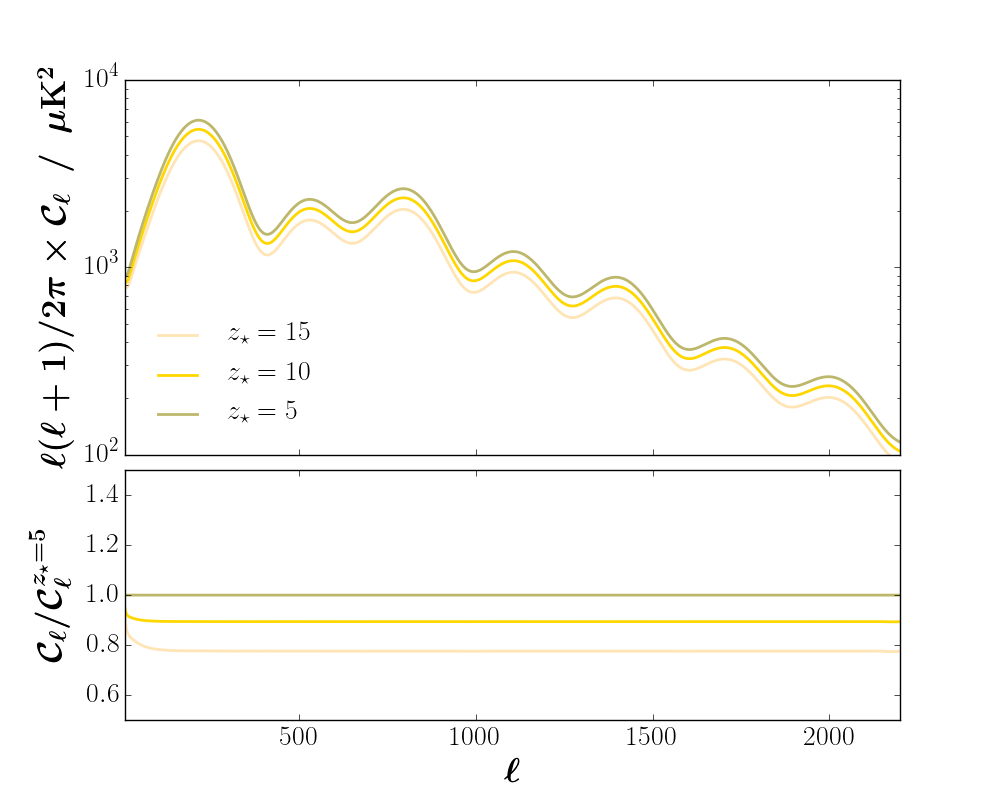
\includegraphics[width=0.45\linewidth]{CosmoParam/Cell_zreio.png}
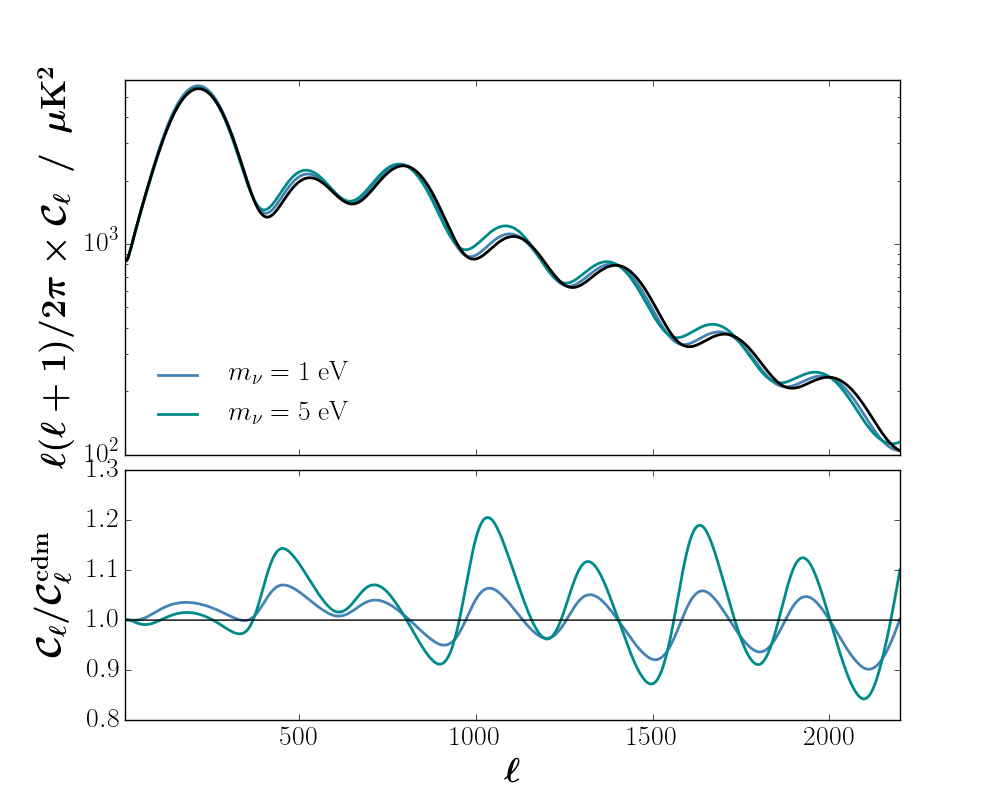
\includegraphics[width=0.65\linewidth]{CosmoParam/Cell_mnu.png}
%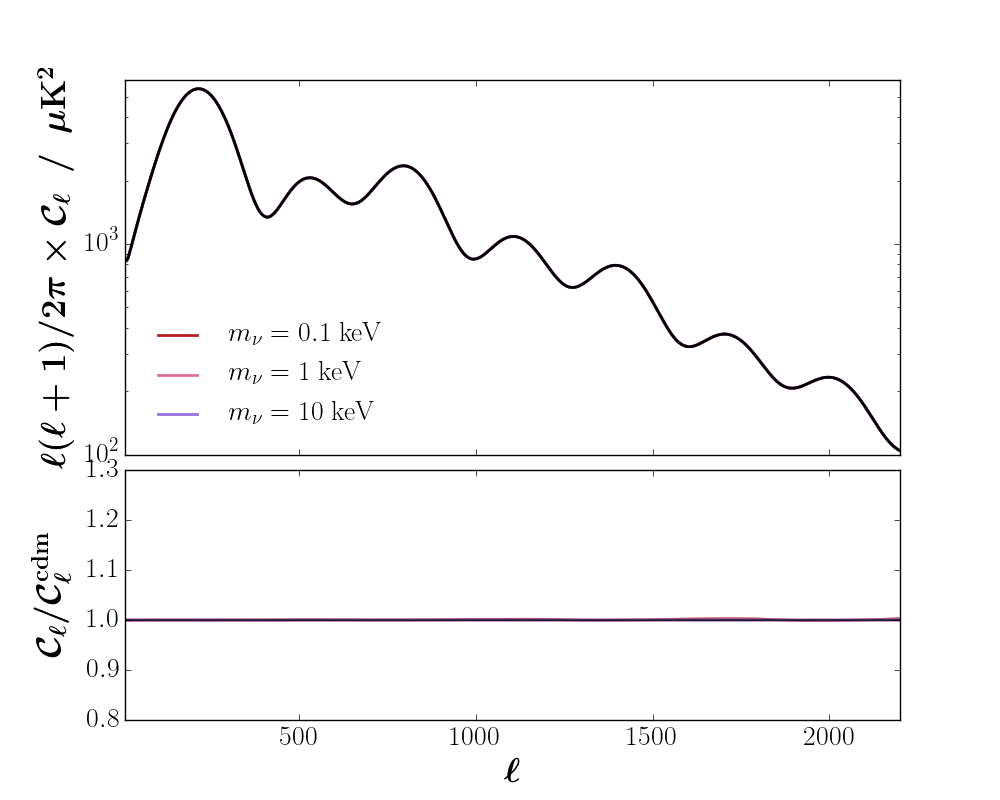
\includegraphics[width=0.45\linewidth]{CosmoParam/Cell_pdm.png}
\caption{Similar caption to Fig.~\ref{fig:Pk_cosmo} for the temperature fluctuation auto-correlation angular power spectrum.}
\label{fig:Cell_cosmo}
\end{center}
\end{figure}

\clearpage